The fundamental goal of the H2020 EU project FAR-EDGE is to devise and develop an Edge computing platform for the virtualization of the factory automation pyramid, in order to support strategically production-related activities during all phases of the engineering and factory life cycle. This objective entails the definition and realization of several software layers serving three high-level functional domains namely, \textit{Automation}, \textit{Analytics}, and \textit{Simulation} (see Figure~\ref{fig:architecture}) to meet the global challenges of mass-customization and reshoring.

\begin{figure}[b]
	\centering
	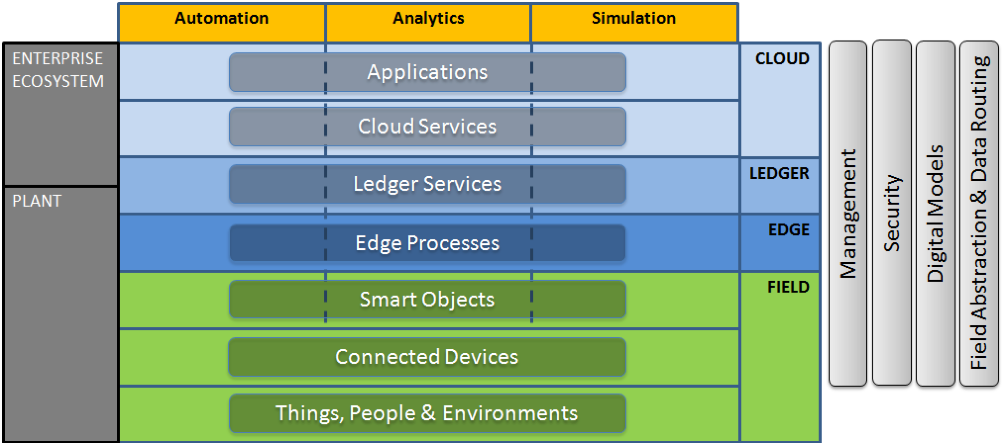
\includegraphics[width=\linewidth]{images/Far-edge.png}
	\caption{FAR-EDGE Reference Architecture overall view}
	\label{fig:architecture}
\end{figure}

As far as simulation is concerned FAR-EDGE aims at providing models and tools entailing functionalities for modeling CPS-based discrete manufacturing factories and simulating their behavior along the whole factory life cycle. 
In the FAR-EDGE vision, in fact, simulation is seen as a first-class citizen of the factory of the future (as it is in I4.0 guidelines), being an enabler to implement layout and product optimization, to test \textit{what-if} scenarios at minimal impact of regular shop activities, or as a the cornerstone to support reactive (\textit{now-what}) operative decisions. 

As was mentioned in the introduction to this chapter, one of the main challenges of simulation in manufacturing is the so-called \textit{Digital Continuity}; it consists in creating the conditions for a model to be up-to-date at any moment during the various phases of the life cycle of a factory. 
Thus, if from one hand this means that the interoperability of the model for virtualization and simulation must be maximized (engineering is by-nature a multidisciplinary process), from the other new mechanisms must be developed and put in place to allow the model to be in-synch with the shop floor evolving as automatically as possible with the state of the factory. As CPSs are subject to changes (e.g., for straining and aging), models should reflect those transformations. To detect this gap and update the model accordingly, raw data from the field (direct) or complex analysis algorithms (from Analytics domain) can be used. However, it is important to point out that the model itself must support model synchronization functionality natively in order to decouple the FAR-EDGE architecture, which must be independent of the particular factory, and the synchronization process that depends on the particular configuration of the factory at hand and ultimately on the model. 
For all the reasons presented above, the task of defining a suitable model is very ambitious; not only FAR-EDGE aims at including in a single harmonic, coherent representation control, communication data collection and simulation data, but also at defining and being able to share a model describing the synchronization process. 

Before being able to present the FAR-EDGE CPS data model and to understand the underlying choices it is important to clarify its relationship with other elements of the reference architecture presented in Figure~\ref{fig:architecture} and in particular with the components related to the simulation domain. 

In Figure~\ref{fig:architectureSimulation} is an excerpt of the overall reference architecture of FAR-EDGE. The simulation domain is envisioned as a layered subsystem of the architecture where the topmost elements are FAR-EDGE-enabled simulation tools and a graphical editor; these rely on the \textit{Open API for Virtualization} to interact with the core of the Simulation subsystem: the CPS Model for Simulation, which is presented in its initial version in this document.

WP4 is responsible for developing and openly providing an API for virtualization that, by means of suitable endpoints allows: 
\begin{itemize}
    \item \textbf{Definition and configuration of simulation scenarios,} including simulation configurations. These will be fully compliant with the FAR-EDGE digital models.
    \item \textbf{Execution of simulation scenarios}, including simulation of CPS systems, machine and devices. FAR-EDGE will support two external simulators in leveraging information and digital models of the inputs and outputs of the CPS systems, along with data mining models and statistics (e.g., time series analysis) that will be used to describe and determine the outputs of the CPS systems during the simulation.
    \item \textbf{Management of digital models synchronization}, including configuration of the Real-to-Digital Synchronization Component and deployment of Synchronization models. 
\end{itemize}


A large number of publications can be found in literature on the topic of simulation; for years, it is considered an established and fundamental tool for the evolution of science. In addition, while with the term simulation we refer to a collection of intuitive concepts, the same is not true for real-to-digital synchronization. For this reason, we dedicate the next section to this topic so that the reader can later easily understand how the data model fulfills the requirement of supporting synchronization.

\begin{figure}
	\centering
	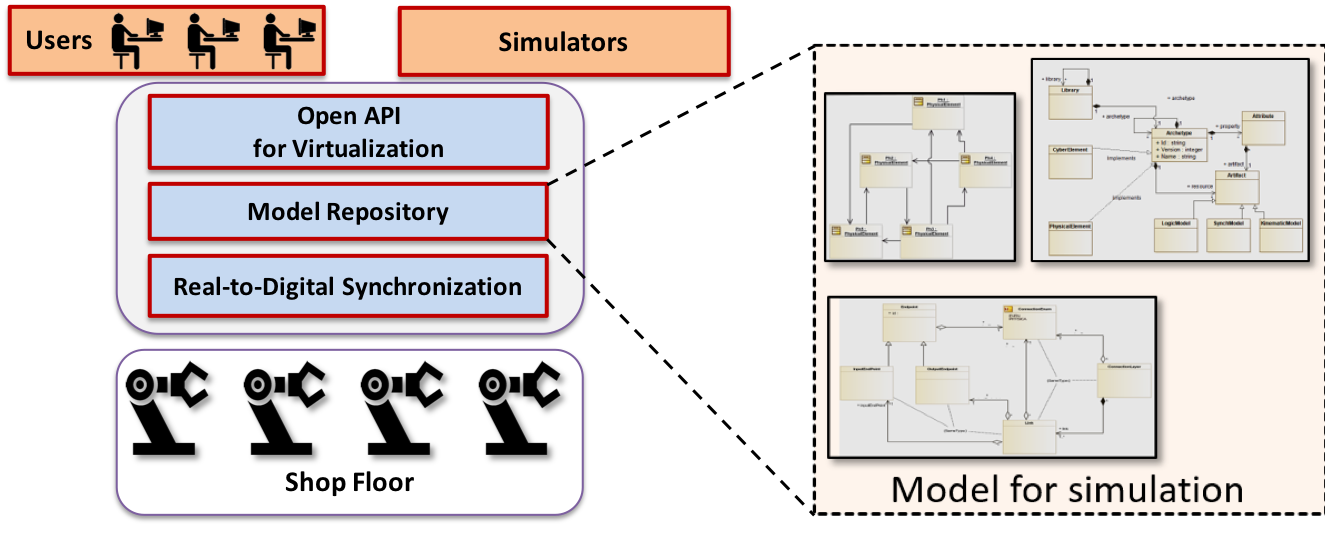
\includegraphics[width=\linewidth]{images/Architecture}
	\caption{Architecture supporting the Digital Continuity}
	\label{fig:architectureSimulation}
\end{figure}

